\section{Kapitel 4}
\subsection{Teilaufgabe 1}
\subsubsection{Aufgabenstellung}
Wir sollen ein Programm schreiben welches Prüft ob zwei Referenzen gleich sind.

\subsubsection{Anforderungsdefinition}
\begin{enumerate}
	\item Prüfe ob zwei Referenzen gleich sind.
\end{enumerate}

\subsubsection{Entwurf}
\begin{center}
	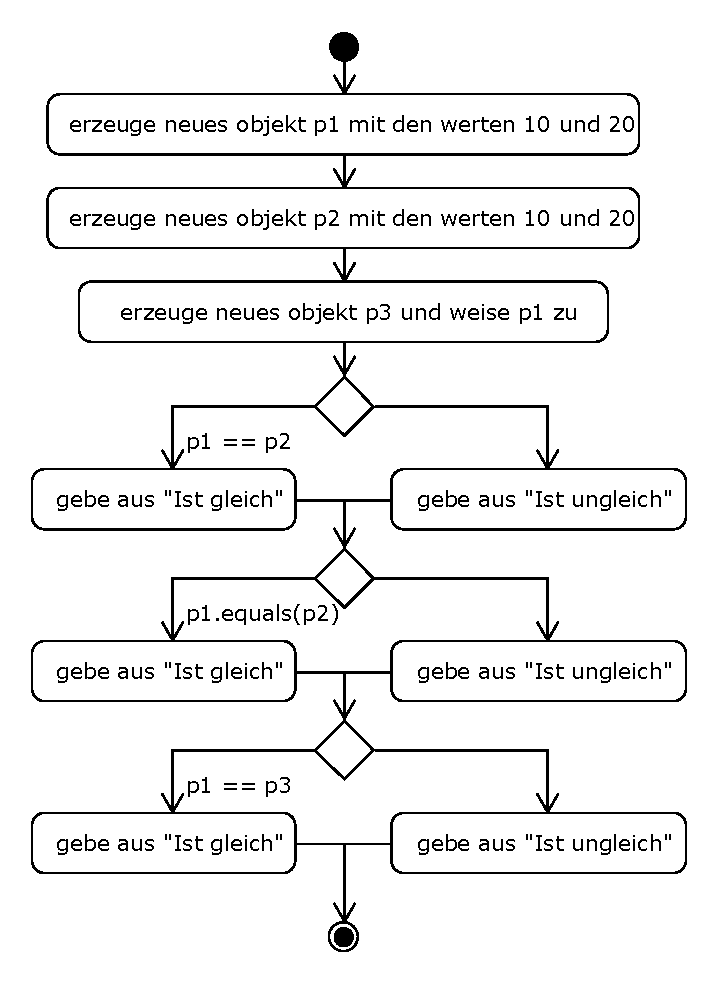
\includegraphics[width=0.7\textwidth]{uml/uml_c4_p1.pdf}
\end{center}

\subsubsection{Quellcode}
\paragraph{Referenzen.java}\
\lstinputlisting[language = Java , frame = trBL , escapeinside={(*@}{@*)}]{../chapter_04/src/main/java/chapter_04/Referenzen.java}
\paragraph{Punkt.java}\
\lstinputlisting[language = Java , frame = trBL , escapeinside={(*@}{@*)}]{../chapter_04/src/main/java/chapter_04/Punkt.java}

\subsubsection{Testdokumentation}
Nach dem Start des Programms sollten die ersten beiden Bedingungen falsch sein und die dritte wahr, dies war auch der Fall.

\subsubsection{Benutzungshinweise}
Navigieren Sie in der Kommandozeile zum dem Ordner, wo sich die Java Datei befindet.
Danach führen sie "javac Referenzen.java\dq \space auf. Jetzt können Sie das Programm mit
"java Referenzen\dq \space starten.

\subsubsection{Anwendungsbeispiel}
Nach dem Aufruf von java Referenzen, sollten wir nun folgendes sehen:
\begin{lstlisting}[frame = trBL , escapeinside={(*@}{@*)}]
[sebastian@laptop bin]$ java Referenzen 
Ist ungleich
Ist ungleich
Ist gleich
[sebastian@laptop bin]$  
\end{lstlisting}
